\documentclass[10pt,letterpaper,twocolumn]{article}

\usepackage[T1]{fontenc}
\usepackage{lmodern}
\usepackage[margin=0.62in,columnsep=0.27in]{geometry}
\usepackage{amsmath,amssymb,mathtools,bm}
\usepackage{array,booktabs,tabularx}
\usepackage{graphicx}
\usepackage{xcolor}
\usepackage{enumitem}
\usepackage{microtype}
\usepackage{fancyhdr}
\usepackage{hyperref}
\usepackage{needspace}
\usepackage{tikz}
\usetikzlibrary{arrows.meta,positioning,calc}

% The user-local tools/array package is newer than the available LaTeX kernel.
\makeatletter
\def\vcenter@text{\vbox}
\makeatother

\graphicspath{{../../../../output/plots/paper_v_results_progression_20260804/}}

\definecolor{navy}{HTML}{17365D}
\definecolor{blue}{HTML}{2B6CB0}
\definecolor{green}{HTML}{2F6B4F}
\definecolor{brick}{HTML}{9B2C2C}
\definecolor{muted}{HTML}{4A5568}

\hypersetup{
  colorlinks=true,
  linkcolor=navy,
  urlcolor=blue,
  citecolor=green,
  pdftitle={From the Archive Equations to the M4 Cone},
  pdfauthor={Local Paper-V learning sequence}
}

\pagestyle{fancy}
\fancyhf{}
\fancyhead[L]{\footnotesize Archive EOM to the fourth-moment cone}
\fancyhead[R]{\footnotesize Paper-V learning sequence}
\fancyfoot[C]{\thepage}
\renewcommand{\headrulewidth}{0.3pt}

\setlength{\parindent}{0pt}
\setlength{\parskip}{3pt plus 0.5pt}
\setlist{nosep,leftmargin=*,topsep=2pt}
\renewcommand{\arraystretch}{1.10}
\newcolumntype{Y}{>{\raggedright\arraybackslash}X}

\newcommand{\R}{\mathbb R}
\newcommand{\C}{\mathbb C}
\newcommand{\I}{\mathbb I}
\newcommand{\ii}{\mathrm i}
\newcommand{\Tr}{\operatorname{Tr}}
\newcommand{\Herm}{\operatorname{Herm}}
\newcommand{\PSD}{\operatorname{PSD}}
\newcommand{\Sym}{\operatorname{Sym}}
\newcommand{\Weyl}{\operatorname{Weyl}}
\newcommand{\diag}{\operatorname{diag}}
\newcommand{\ket}[1]{\lvert #1\rangle}
\newcommand{\bra}[1]{\langle #1\rvert}
\newcommand{\braket}[2]{\langle #1\mid #2\rangle}
\newcommand{\expect}[1]{\left\langle #1\right\rangle}
\newcommand{\dd}{\,\mathrm d}
\newcommand{\sectionline}[1]{%
  \Needspace{6\baselineskip}%
  \par\medskip{\color{navy}\large\bfseries #1}\par
  \vspace{-2pt}{\color{navy}\rule{\columnwidth}{0.7pt}}\par\smallskip
}
\newcommand{\conceptbreak}{%
  \par\medskip\noindent
  {\color{black!28}\rule{\columnwidth}{0.35pt}}%
  \par\medskip
}

\begin{document}
\raggedbottom

\twocolumn[
\begin{center}
  {\color{navy}\LARGE\bfseries From the Archive Equations to the $M_4$ Cone}\par\vspace{3pt}
  {\Large Physical moment hierarchies, positive completion, and cone slicing}\par\vspace{4pt}
  {\small A construction-first route through the matched Paper-V result, 5 August 2026}
\end{center}
\vspace{3pt}\hrule\vspace{7pt}
]

\begin{abstract}
The archive equal-time equations propagate five reduced objects
\(X=(\rho,B,N,A,C)\).  Their closure is executable, yet its finite state does
not carry every higher expectation requested by the exact Heisenberg
hierarchy.  The $M_4$ route inserts a degree-complete Pauli--Weyl layer through
degree three, supplies its degree-four frontier by a positive moment
completion, and keeps that enlarged moment matrix feasible at every accepted
SSPRK stage.  In the matched strong-coupling calculation through
\(t t_{\rm hop}=4\), this construction reduces the 31-scalar time-RMS error
from \(0.04995\) for the unconstrained higher-moment prior to \(0.01258\), and
reduces total-internal-energy RMS error from \(0.02509\) to
\(8.21\times10^{-4}\).  The improvement identifies the positive fourth-moment
completion as an active closure mechanism in this test.  It does not establish
exact reduced dynamics, long-time transfer, or a general closure theorem.
\end{abstract}

\sectionline{The governing calculation}

The route begins with the driven Holstein dimer and ends with observables that
can be compared against an exact cutoff-16 wavefunction only after the
autonomous reduced propagation is complete:
\[
\begin{gathered}
H(t),\ \ket{\Psi(0)}
\longrightarrow
\underbrace{X=(\rho,B,N,A,C)}_{\text{archive moments}},\\
X\longrightarrow
\underbrace{x_{\rm raw}\in\R^{29}}_{\text{exact structural chart}},\\
x_{\rm raw}\oplus\eta_{\le3}\in\R^{60}
\xrightarrow{\ \dot x=f_{\rm arch}+f_{KPD}\ }
\dot x,\\
\eta_{\le3}
\xrightarrow{\text{degree-four completion}}
M_4\succeq0
\xrightarrow{\text{stage containment}}
x(t),\\
x(t)\xrightarrow{\text{contraction}}\mathcal O(t),\\
\mathcal O(t)\xrightarrow{\text{offline score}}\text{RMS errors}.
\end{gathered}
\tag{1}
\]
The scored tuple is
\[
\mathcal O=(n_0,n_1,E_{\rm e},E_{\rm ph},E_{\rm e-ph},E_{\rm int}).
\]
Here \(\eta_{\le3}\in\R^{31}\) contains six electronic two-spin moments and
all twenty-five degree-three moments absent from the 29-coordinate raw chart.
The symbol \(M_4\) denotes a 33-by-33 Gram matrix whose entries require moments
through degree four.  It is a matrix assembled from moments; it is not the set
of fourth moments alone.

The shortest reading path is Sections 1--8 followed by the companion problem
workbook.  During the first pass, keep Eq.~(1) visible.  After Section 8, close
the source and reconstruct the map from the Hamiltonian to the RMS table before
attempting any local formula.

\sectionline{1. The dimer before reduction}

For two electronic sites \(i\in\{0,1\}\), two spin channels
\(s\in\{\uparrow,\downarrow\}\), and two local phonons, the joint state lives
in the fixed-particle sector of
\[
\mathcal H=\mathcal F_{\rm e}\otimes\mathcal F_{\rm ph}.
\tag{2}
\]
Fermionic operators satisfy
\(\{c_{is},c_{js'}^\dagger\}=\delta_{ij}\delta_{ss'}\); phonon operators
satisfy \([b_i,b_j^\dagger]=\delta_{ij}\).  The driven local-Holstein
Hamiltonian is
\[
\begin{aligned}
H(t)={}&-t_{\rm hop}\sum_s
\left(c_{0s}^\dagger c_{1s}+c_{1s}^\dagger c_{0s}\right)\\
&+\omega_{\rm ph}\sum_i b_i^\dagger b_i
+g\sum_{i,s}(b_i+b_i^\dagger)n_{is}+H_{\rm ext}(t),
\end{aligned}
\tag{3}
\]
where \(n_{is}=c_{is}^\dagger c_{is}\).  Hopping moves electronic amplitude
between sites, the phonon term rotates oscillator phase, and the local coupling
makes site occupation act as a force on the local displacement.

The matched result uses
\[
t_{\rm hop}=1,\qquad
\gamma=\frac{\omega_{\rm ph}}{t_{\rm hop}}=0.5,\qquad
\lambda=\frac{2g^2}{t_{\rm hop}\omega_{\rm ph}}=1.5,
\tag{4}
\]
so \(g/t_{\rm hop}=0.612372\ldots\).  The single Gaussian pulse has unit
amplitude and unit width.  The phonon cutoff is 16.

\conceptbreak
\textbf{Center and relative phonons.}
The orthogonal mode transformation
\[
b_+=\frac{b_0+b_1}{\sqrt2},\qquad
b_-=\frac{b_0-b_1}{\sqrt2}
\tag{5}
\]
separates a coherent center oscillator from the interacting relative
oscillator in the fixed one-up/one-down sector.  Define the relative
quadratures
\[
x=\frac{b_-+b_-^\dagger}{\sqrt2},\qquad
p=\frac{b_--b_-^\dagger}{\ii\sqrt2},\qquad [x,p]=\ii.
\tag{6}
\]
Each spin channel carries one electron over two sites and is therefore a
two-level system.  Pauli matrices \(X_s,Y_s,Z_s\) act on that site qubit.  Up
to the separately propagated coherent center energy, the active relative-mode
Hamiltonian has the form implemented by the moment hierarchy,
\[
\begin{aligned}
H_-(t)={}&-t_{\rm hop}(X_\uparrow+X_\downarrow)
+\frac{\Delta(t)}{2}(Z_\uparrow+Z_\downarrow)\\
&+\frac{\omega_{\rm ph}}{2}(x^2+p^2)
+g\,x(Z_\uparrow+Z_\downarrow).
\end{aligned}
\tag{7}
\]
The pulse enters through the site-energy difference \(\Delta(t)\).  Equation
(7) is the compact physical engine of the hierarchy: the term \(gxZ_s\)
multiplies an electronic operator by one oscillator quadrature and can raise a
moment's total degree.

\sectionline{2. The Heisenberg equation creates the hierarchy}

Let \(O\) be a time-independent operator and
\(\ket{\Psi(t)}\) obey \(\ii\partial_t\ket{\Psi}=H\ket{\Psi}\).  Differentiating
its expectation gives
\[
\begin{aligned}
\frac{\dd}{\dd t}\expect{O}
&=\frac{\dd}{\dd t}\bra{\Psi}O\ket{\Psi}\\
&=\bra{\dot\Psi}O\ket{\Psi}+\bra{\Psi}O\ket{\dot\Psi}\\
&=\ii\bra{\Psi}HO\ket{\Psi}
-\ii\bra{\Psi}OH\ket{\Psi}\\
&=\ii\expect{[H,O]}.
\end{aligned}
\tag{8}
\]
An explicitly time-dependent operator would add
\(\expect{\partial O/\partial t}\).  Every moment equation in the hierarchy is
Eq.~(8) evaluated for a different \(O\).

The oscillator primitives close among themselves under the quadratic phonon
Hamiltonian:
\[
\begin{aligned}
\dot{\expect{x}}
&=\ii\expect{[H_-,x]}
=\omega_{\rm ph}\expect{p},\\
\dot{\expect{p}}
&=\ii\expect{[H_-,p]}
=-\omega_{\rm ph}\expect{x}
-g\expect{Z_\uparrow+Z_\downarrow}.
\end{aligned}
\tag{9}
\]
The first line follows from \([p^2,x]=-2\ii p\); the second uses
\([x^2,p]=2\ii x\) and \([xZ_s,p]=\ii Z_s\).  The oscillator receives a force
from electronic imbalance.

Electronic motion immediately exposes the upward chain.  Since
\([X,Z]=-2\ii Y\) and \([Z,Y]=-2\ii X\),
\[
\begin{aligned}
\dot{\expect{Z_s}}
&=-2t_{\rm hop}\expect{Y_s},\\
\dot{\expect{Y_s}}
&=2t_{\rm hop}\expect{Z_s}
+\Delta(t)\expect{X_s}
+2g\expect{xX_s}.
\end{aligned}
\tag{10}
\]
The one-spin moment \(\expect{Y_s}\) therefore requests the mixed degree-two
moment \(\expect{xX_s}\).  Differentiating that requested moment yields
\[
\begin{aligned}
\frac{\dd}{\dd t}\expect{xX_s}
={}&\omega_{\rm ph}\expect{pX_s}
-\Delta(t)\expect{xY_s}
-2g\expect{x^2Y_s},
\end{aligned}
\tag{11}
\]
which requests a degree-three moment.  Repeating the operation gives
\[
\expect{Y_s}\longrightarrow
\expect{xX_s}\longrightarrow
\expect{x^2Y_s}\longrightarrow\cdots .
\tag{12}
\]
The hierarchy is thus a consequence of operator multiplication under the
commutator.  It is present before coordinates, numerical integration, or a
closure rule are chosen.

\sectionline{3. Pauli--Weyl moments make the hierarchy degree-complete}

For Pauli labels \(\alpha,\beta\in\{I,X,Y,Z\}\) and nonnegative integers
\(m,n\), define the Hermitian Weyl moment
\[
\mu_{\alpha\beta mn}(t)
=\expect{\sigma_\alpha^\uparrow\sigma_\beta^\downarrow
\Weyl(x^m p^n)}_t.
\tag{13}
\]
Weyl ordering symmetrizes every distinct ordering of the \(m\) factors of
\(x\) and \(n\) factors of \(p\).  It turns noncommuting operator polynomials
into a real coordinate family for Hermitian moments.

The total degree is
\[
d(\alpha,\beta,m,n)
=\mathbf1_{\alpha\ne I}+\mathbf1_{\beta\ne I}+m+n.
\tag{14}
\]
The degree-three symmetry-adapted hierarchy retains 5 degree-one, 15
degree-two, and 25 degree-three moments.  Together with the real and imaginary
parts of the decoupled center amplitude, its direct hierarchy chart would have
47 real coordinates.  The APCM entrance layer uses a different, overlapping
chart: 29 structurally independent raw archive moments plus 31 hidden moments,
for 60 real coordinates.

The product of Weyl monomials follows the Moyal product.  Its leading terms are
\[
f\star g
=fg+\frac{\ii}{2}
\left(\partial_xf\,\partial_pg-\partial_pf\,\partial_xg\right)+\cdots .
\tag{15}
\]
Combining Eq.~(15) with
\(\sigma_a\sigma_b=\delta_{ab}I+\ii\sum_c\epsilon_{abc}\sigma_c\)
reduces every commutator in Eq.~(8) to other Pauli--Weyl moments.  Under
Eq.~(7), a retained degree-three equation can request degree-four moments.  A
finite autonomous model must therefore say how those degree-four values are
chosen.

\conceptbreak
\textbf{Cumulant closure.}
Cumulants isolate the connected part of a moment.  For three commuting
placeholders \(A,B,C\),
\[
\begin{aligned}
\expect{ABC}
={}&\kappa(A,B,C)
+\kappa(A,B)\expect C
+\kappa(A,C)\expect B\\
&+\kappa(B,C)\expect A
+\expect A\expect B\expect C.
\end{aligned}
\tag{16}
\]
The zero-terminal-cumulant rule sets the first omitted connected cumulant to
zero and reconstructs the raw moment from all lower-order partitions.  At a
degree-three truncation, it proposes every requested degree-four moment from
moments of degree at most three.  This produces a deterministic frontier
\(m_4^{(0)}\), called the zero-cumulant prior below.  Matching the required
output shape makes the ODE executable; it supplies no representability or
accuracy theorem.

\sectionline{4. Where the archive tuple sits inside the hierarchy}

The archive equations retain five equal-time objects:
\[
\begin{array}{rcll}
\rho_{ij}&=&\expect{c_j^\dagger c_i},
&\rho\in\Herm(2),\\
B_q&=&\expect{b_q},&B\in\C^2,\\
N_{qq'}&=&\expect{\delta b_{q'}^\dagger\delta b_q},
&N\in\Herm(2),\\
A_{qq'}&=&\expect{\delta b_q\delta b_{q'}},
&A\in\Sym_2(\C),\\
C^q_{ij}&=&\expect{\delta b_q c_j^\dagger c_i}_{\!c},
&C\in\C^{2\times2\times2},
\end{array}
\tag{17}
\]
where \(\delta b_q=b_q-B_q\), and the subscript \(c\) denotes the connected
part after products already represented by \(B\) and \(\rho\) are removed.
The five sectors contain coherent phonons, bosonic second moments, electronic
one-body information, and one-phonon electron correlations.

Their matrix vector field has the dependency structure
\[
\begin{array}{rcl}
\dot\rho&=&F_\rho(\rho,B,C),\\
\dot B&=&F_B(B,\rho),\\
\dot N&=&F_N(N,C),\\
\dot A&=&F_A(A,C),\\
\dot C&=&F_C(C;\rho,B,N,A).
\end{array}
\tag{18}
\]
The semicolon records that the archive correlation equation is linear in
\(C\) along a prescribed history of the other objects.  The simultaneous
system remains nonlinear because those objects coevolve.

For example, the coherent phonon is a forced oscillator,
\[
\dot B_q=-\ii\omega_qB_q
-\ii s\sum_{ij}(G_q)_{ij}\rho_{ij},
\tag{19}
\]
and the electronic density contains coherent transport and correlation
feedback,
\[
\dot\rho=-\ii[\widetilde h,\rho]+\Phi_C+\Phi_C^\dagger.
\tag{20}
\]
The normal and anomalous boson moments receive sources linear in \(C\).  The
correlation equation transports existing \(C\) and creates new \(C\) from
products of \(\rho,N,A\).  Those products are the archive closure of the
higher moments exposed by Eq.~(8).

The familiar 31-real chart counts
\[
\underbrace{3}_{\rho}
+\underbrace{4}_{B}
+\underbrace{4}_{N}
+\underbrace{6}_{A}
+\underbrace{14}_{C}=31.
\tag{21}
\]
The 31-real archive chart already enforces the weaker shared-trace condition
\(\Tr C^0=\Tr C^1\), leaving one shared complex trace.  The APCM entrance
layer specializes to individually traceless centered correlations,
\(\Tr C^0=\Tr C^1=0\).  Setting that remaining shared complex trace to zero
removes two further real coordinates, so the raw chart stores 29 independent
moments.  It then adds 31 hidden Pauli--Weyl moments:
six two-spin electronic moments and all twenty-five degree-three moments.

\conceptbreak
\textbf{The $K/P/D$ correction.}
The augmented correlation velocity takes the form
\[
\dot C_{\rm aug}=\dot C_{\rm arch}+\Delta\dot C_K
+\Delta\dot C_P+\Delta\dot C_D.
\tag{22}
\]
The \(K\) term carries connected electron--two-phonon information decoded from
the degree-three moments; \(P\) is the verified same-spin Pauli replacement of
the archive source; \(D\) carries opposite-spin electronic covariance.  These
terms repair an identified local defect in the archive \(C\)-velocity.  They
do not close the degree-three hierarchy by themselves: the derivative of the
new degree-three state still requests degree-four moments.

\sectionline{5. A moment cone is forced by positive quantum squares}

Choose a finite ordered word list
\(\mathcal W=(W_1,\ldots,W_d)\) and form an arbitrary operator combination
\(Q(z)=\sum_a z_aW_a\), with \(z\in\C^d\).  Quantum positivity gives
\[
0\le\expect{Q(z)^\dagger Q(z)}
=\sum_{ab}z_a^*\expect{W_a^\dagger W_b}z_b
=z^\dagger M(\mu)z,
\tag{23}
\]
where
\[
M(\mu)_{ab}=\expect{W_a^\dagger W_b}.
\tag{24}
\]
Since Eq.~(23) holds for every \(z\), every physical set of moments must obey
\(M(\mu)\succeq0\).  This is a necessary representability condition.  The
moment matrix is a Gram matrix in the state-dependent inner product
\((A,B)_\Psi=\expect{A^\dagger B}\).

The retained archive variables yield a 7-by-7 joint electron--phonon Gram
matrix of the schematic block form
\[
\mathcal G(X)=
\begin{pmatrix}
M_{\rm B}(N,A)&Z(C)\\
Z(C)^\dagger&E(\rho)
\end{pmatrix}\succeq0.
\tag{25}
\]
Its diagonal blocks test bosonic and electronic fluctuations.  Its
off-diagonal block tests whether the retained correlation \(C\) can coexist
with those marginal fluctuations.  The Schur complement reads, on supported
electronic directions,
\[
M_{\rm B}-Z E^+ Z^\dagger\succeq0.
\tag{26}
\]
Equation~(26) is the operator Cauchy--Schwarz budget: marginal variances limit
the size and orientation of their joint correlation.

\sectionline{6. Constructing the extended $M_4$ cone}

For the extended test, \(\mathcal W_{\le2}\) contains every implemented
Pauli--Weyl word of degree at most two needed by the spin-symmetric dimer:
the identity, eight degree-one words, and twenty-four degree-two words.  Thus
\(d=33\).  Its Gram matrix is
\[
[M_4]_{ab}=\expect{W_a^\dagger W_b},
\qquad W_a,W_b\in\mathcal W_{\le2}.
\tag{27}
\]
Products of two degree-two words reach degree four, so Eq.~(27) is affine in
all moments through degree four:
\[
M_4(\mu_{\le3},m_4)
=M_{\rm fixed}(\mu_{\le3})
+\sum_{k=1}^{35}(m_4)_kF_k.
\tag{28}
\]
The 35-vector \(m_4\) contains the symmetry-adapted degree-four frontier, and
each Hermitian coefficient matrix \(F_k\) records where that moment appears in
the word Gram matrix.

The zero-cumulant rule supplies a prior \(m_4^{(0)}\).  The positive completion
chooses a nearby frontier inside the cone:
\[
\begin{aligned}
\underset{m_4\in\R^{35}}{\operatorname{minimize}}\quad
&\frac12\left\|S_4^{-1}(m_4-m_4^{(0)})\right\|_2^2
-\tau\log\det(M_4+\epsilon I)\\
\text{subject to}\quad
&M_4(\mu_{\le3},m_4)\succeq0,\\
&-4s_k\le(m_4)_k\le4s_k.
\end{aligned}
\tag{29}
\]
The diagonal scale matrix \(S_4=\diag(s_1,\ldots,s_{35})\) increases with
boson degree and the declared phonon envelope.  The first objective term keeps
the frontier near its cumulant prior.  The logarithmic determinant selects a
nonsingular interior representative when the feasible set permits one.  The
bounds prevent uncontrolled terminal moments.  Equation~(29) is the operation
called positive fourth-moment completion.

At an intermediate SSPRK stage, the lower moments can move enough that the
previous frontier ceases to certify Eq.~(27).  The stage retraction holds the
29 raw archive coordinates fixed and changes only the 31 hidden lower moments,
with a weak frontier regularizer:
\[
\begin{aligned}
\underset{\eta',m_4}{\operatorname{minimize}}\quad
&\frac12\|S_\eta^{-1}(\eta'-\eta)\|_2^2
+10^{-8}\|S_4^{-1}(m_4-m_4^{\rm warm})\|_2^2\\
\text{subject to}\quad
&M_4(\mu_{\rm raw},\eta',m_4)\succeq0.
\end{aligned}
\tag{30}
\]
This makes the $M_4$ cone dynamically active twice: it selects the terminal
degree-four values used in the degree-three velocity, and it contains the
accepted lower-moment stages inside an extendable moment sequence.

\begin{figure*}[t]
\centering
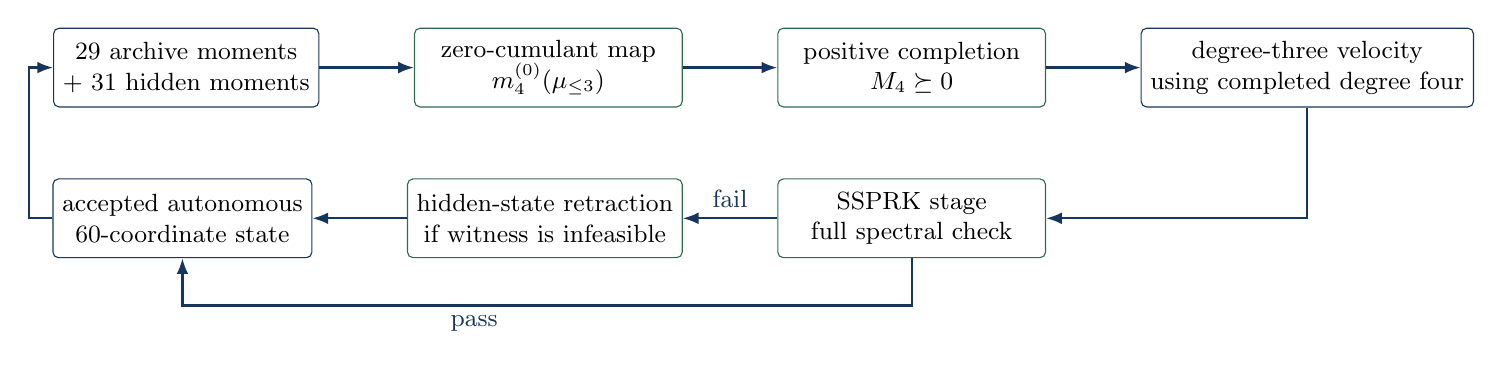
\begin{tikzpicture}[
  node distance=9mm and 12mm,
  every node/.style={font=\small,align=center},
  state/.style={draw=navy,rounded corners=2pt,minimum width=31mm,minimum height=10mm},
  op/.style={draw=green,rounded corners=2pt,minimum width=34mm,minimum height=10mm},
  arr/.style={-{Latex[length=2mm]},thick,navy}
]
\node[state] (lower) {29 archive moments\\+ 31 hidden moments};
\node[op,right=of lower] (prior) {zero-cumulant map\\\(m_4^{(0)}(\mu_{\le3})\)};
\node[op,right=of prior] (complete) {positive completion\\\(M_4\succeq0\)};
\node[state,right=of complete] (velocity) {degree-three velocity\\using completed degree four};
\node[op,below=of complete] (stage) {SSPRK stage\\full spectral check};
\node[op,left=of stage] (retract) {hidden-state retraction\\if witness is infeasible};
\node[state,left=of retract] (accepted) {accepted autonomous\\60-coordinate state};
\draw[arr] (lower) -- (prior);
\draw[arr] (prior) -- (complete);
\draw[arr] (complete) -- (velocity);
\draw[arr] (velocity.south) |- (stage.east);
\draw[arr] (stage.west) -- node[above]{fail} (retract.east);
\draw[arr] (retract.west) -- (accepted.east);
\draw[arr] (stage.south) -- ++(0,-6mm)
  -| node[pos=0.30,below]{pass} (accepted.south);
\draw[arr] (accepted.west) -- ++(-3mm,0) |- (lower.west);
\end{tikzpicture}
\caption{The positive-completion loop.  The degree-four frontier is selected
from the current degree-three state, used in the hierarchy velocity, and
rechecked after every SSPRK stage.  Retraction changes hidden lower moments
only when the warm frontier no longer supplies a feasible $M_4$ witness.}
\label{fig:m4loop}
\end{figure*}

\sectionline{7. Cone slicing derives a minimum correction}

The retained controller and the $M_4$ completion share positive-semidefinite
geometry, yet they solve different problems.  The retained controller chooses
an additive velocity correction \(w\in\R^{31}\).  Let
\(B_\ell(w)\) be one affine barrier matrix, with
\(\ell\in\{\rho^-,\rho^+,\mathcal G\}\):
\[
\begin{aligned}
B_{\rho^-}(w)&=\dot\rho+\Delta\dot\rho(w)
+\beta(\rho-h_\star I),\\
B_{\rho^+}(w)&=-\dot\rho-\Delta\dot\rho(w)
+\beta(I-\rho-h_\star I),\\
B_{\mathcal G}(w)&=\dot{\mathcal G}+\Delta\dot{\mathcal G}(w)
+\beta(\mathcal G-h_\star I).
\end{aligned}
\tag{31}
\]
The inequalities \(B_\ell(w)\succeq0\) require inward velocity at a cone
boundary and permit bounded outward motion in the interior.  The rate
\(\beta>0\) sets the desired recovery law; \(h_\star\ge0\) is the safety
margin.

Energy neutrality and the fixed-number correlation trace give linear
equalities
\[
Lw=d.
\tag{32}
\]
After transforming into the selected correction metric, compute the
minimum-norm particular solution \(w_{\rm p}\) and an orthonormal null basis
\(Z\):
\[
Lw_{\rm p}=d,\qquad LZ=0,\qquad
w=w_{\rm p}+Zy.
\tag{33}
\]
Every reduced coordinate \(y\) now satisfies the equalities.  The remaining
task is the nearest point satisfying all matrix inequalities.

Suppose the complete matrix \(B_\ell(w_{\rm p}+Zy^{(k)})\) has a negative
eigenpair
\[
B_\ell(w_{\rm p}+Zy^{(k)})v=\lambda v,\qquad
v^\dagger v=1,\qquad\lambda<0.
\tag{34}
\]
For the standard correction vector \(e_j\in\R^{31}\), define the exposed-mode
sensitivity
\[
a_j=v^\dagger\Delta B_\ell(e_j)v,
\qquad n=Z^{\mathsf T}a.
\tag{35}
\]
The scalar \(a_j\) is the change in the tested barrier quadratic form per unit
correction coordinate.  Because \(B_\ell\) is affine in \(w\), holding this
matrix direction \(v\) fixed gives the exact relation
\[
v^\dagger B_\ell(w_{\rm p}+Zy)v
=\lambda+n^{\mathsf T}(y-y^{(k)}).
\tag{36}
\]
The exposed negative direction therefore yields the half-space
\[
n^{\mathsf T}y\ge n^{\mathsf T}y^{(k)}-\lambda.
\tag{37}
\]
Every semidefinite-feasible correction lies in this half-space.  One cut tests
one direction \(v\); it does not certify the other directions of the complete
matrix.

After \(p\) exposed modes, solve
\[
\begin{aligned}
\underset{y}{\operatorname{minimize}}\quad&\frac12y^{\mathsf T}y\\
\text{subject to}\quad&n_i^{\mathsf T}y\ge c_i,
\qquad i=1,\ldots,p.
\end{aligned}
\tag{38}
\]
Then reconstruct \(w\), rebuild every complete barrier matrix, diagonalize
again, and add each newly negative direction.  The cycle
\[
y^{(k)}\longrightarrow B_\ell
\longrightarrow(\lambda,v)
\longrightarrow(n^{\mathsf T}y\ge c)
\longrightarrow y^{(k+1)}
\tag{39}
\]
terminates only when all full spectra pass the cone tolerance.  Near a
degenerate face, the implementation can fall back to direct eigenvalue
constraints initialized from the accumulated-cut solution.

For one inequality \(a^{\mathsf T}w+\lambda\ge0\) with no equalities and
\(\lambda<0\), the Lagrangian
\[
\mathcal L(w,\mu)=\frac12w^{\mathsf T}w
-\mu(a^{\mathsf T}w+\lambda)
\tag{40}
\]
gives \(w=\mu a\).  Complementarity makes the active inequality an equality,
so
\[
\mu=-\frac{\lambda}{a^{\mathsf T}a},\qquad
w^\star=-\frac{\lambda}{a^{\mathsf T}a}a.
\tag{41}
\]
Equation~(41) explains the first cut geometrically: move along the exposed
mode's response normal by exactly the distance needed to reach its supporting
hyperplane.  Subsequent cuts change the nearest feasible direction.

\begin{table*}[t]
\centering
\small
\begin{tabularx}{0.95\textwidth}{@{}lYYY@{}}
\toprule
Construction & Chosen variable & Positive matrix & Role in the $M_4$ result\\
\midrule
Retained cone slicing
& additive 31-coordinate velocity \(w\)
& \(\rho\), \(I-\rho\), and retained \(\mathcal G(X)\)
& keeps selected archive moments inside necessary marginal and joint cones\\
Positive fourth-moment completion
& 35 degree-four frontier moments \(m_4\)
& 33-by-33 word Gram matrix \(M_4(\mu_{\le3},m_4)\)
& supplies terminal moments used by the degree-three hierarchy\\
Hidden-stage retraction
& 31 hidden lower moments \(\eta\), with a weakly adjusted frontier
& the same extended \(M_4\)
& contains each accepted SSPRK stage inside the extendable moment cone\\
\bottomrule
\end{tabularx}
\caption{Three cone operations that must remain distinct.  They act on
different variables and enter the autonomous calculation at different points.}
\label{tab:cones}
\end{table*}

\sectionline{8. Reading the matched $M_4$ result}

Figure~\ref{fig:matched} compares exact cutoff-16 Hamiltonian propagation,
the raw archive EOM, the retained-cone archive EOM, and four factorial cells of
the higher-moment route.  Every higher-moment cell uses the same 60-coordinate
initial state, Hamiltonian, pulse, cutoff, \(h=0.0025\), and SSPRK(3,3)
protocol.  The two switches are the retained joint-Gram controller and the
extended $M_4$ completion/retraction.

\begin{figure*}[t]
\centering
\includegraphics[width=0.93\textwidth]{apcm_t4_matched_observables.pdf}
\caption{Matched strong-coupling trajectories through
\(t t_{\rm hop}=4\).  Black is exact cutoff-16 propagation.  The close green
and blue curves use positive $M_4$ completion without and with the retained
joint-Gram controller.  Exact trajectory data enter only after autonomous
rollout for scoring.  Source: the first page of the Paper-V results progression
record dated 4--5 August 2026.}
\label{fig:matched}
\end{figure*}

\begin{table*}[t]
\centering
\small
\setlength{\tabcolsep}{4pt}
\begin{tabular}{@{}lrrrrrr@{}}
\toprule
Model & 31 RMS & \(C\) RMS & \(n_0\) RMS & \(E_{\rm int}\) RMS
& \(\min\lambda(\mathcal G)\) & \(\min\lambda(M_4)\)\\
\midrule
Higher moment: no cones
& 0.04995 & 0.10663 & 0.04806 & 0.02509
& \(-8.23\times10^{-3}\) & \(-1.487\)\\
Higher moment + retained cone
& 0.04647 & 0.10323 & 0.05179 & 0.02697
& \(1.03\times10^{-5}\) & \(-1.473\)\\
Higher moment + \(M_4\) cone
& 0.01258 & 0.04743 & 0.01512 & \(8.21\times10^{-4}\)
& \(2.89\times10^{-5}\) & \(-9.68\times10^{-7}\)\\
Higher moment + both cones
& 0.01258 & 0.04725 & 0.01385 & \(7.96\times10^{-4}\)
& \(2.89\times10^{-5}\) & \(-8.76\times10^{-7}\)\\
\bottomrule
\end{tabular}
\caption{Time-RMS errors over \(0\le t t_{\rm hop}\le4\).  The small negative
extended-cone minima lie within the declared \(10^{-6}\) conic backward-error
tolerance.}
\label{tab:m4result}
\end{table*}

Three deductions follow from the matched cells.

First, the retained controller performs its declared task.  It moves
\(\min\lambda(\mathcal G)\) from \(-8.23\times10^{-3}\) to a positive value
when the terminal prior remains unchanged.  The aggregate and energy errors do
not improve materially in that pair.  Retained representability and trajectory
accuracy are distinct validity axes.

Second, positive $M_4$ completion changes the autonomous dynamics.  With the
retained controller off, it reduces 31-scalar RMS error by a factor of 3.97,
\(C\)-block RMS error by a factor of 2.25, and total-internal-energy RMS error
by a factor of 30.6 relative to the no-cone higher-moment cell.  The mechanism
is larger than passive certification: completed degree-four moments enter the
degree-three velocity, and retraction changes hidden stages when needed.

Third, the two positive-completion cells nearly coincide over this horizon.
The $M_4$-only cell remains inside the retained joint cone even though that
controller is disabled.  This observed redundancy is protocol-local.  It does
not prove that \(M_4\succeq0\) always implies the specific retained controller
constraints under every truncation, state chart, or numerical tolerance.

The computational cost is consequential.  The no-cone cell takes 27.3 s, the
retained-only cell 52.1 s, the $M_4$-only cell 3268.6 s, and the both-cones cell
3399.6 s.  A spin-exchange block diagonalization of the 33-by-33 cone yields
exact 21-by-21 and 12-by-12 blocks, yet a faster block-solver candidate produced
different near-degenerate retraction solutions and failed full trajectory
parity.  The serial full-cone semantics therefore remain the result authority.

\sectionline{9. What the result establishes}

The matched calculation establishes the following bounded statement.  For the
specified strong-coupling dimer, exact-correlated initialization, cutoff 16,
single pulse, 60-coordinate entrance layer, fixed SSPRK(3,3) step, and horizon
\(t t_{\rm hop}\le4\), a positive degree-four completion plus hidden-stage
containment produces much smaller retained-moment and observable errors than
the same higher-moment vector field with its zero-cumulant terminal prior.

The result leaves four scientific questions open.

\begin{enumerate}
\item \textbf{Dynamical completeness.}  A positive truncated sequence can
still differ from the exact hierarchy because positivity is a necessary
representability condition, not the missing exact closure law.
\item \textbf{Long-time transfer.}  The matched $M_4$ ablation ends at
\(t t_{\rm hop}=4\).  Later packet-state results address longer horizons with
a different propagated object.
\item \textbf{Model transfer.}  Other couplings, drives, preparations, and
phonon cutoffs can expose different moment directions.
\item \textbf{Efficient conic realization.}  A faster optimizer must preserve
the selected state and cone trajectory, not only the formal feasible set.
\end{enumerate}

The central physical lesson is compact.  The archive closure retains a useful
low-order subsystem.  Its equations request higher correlations that were
factorized.  The degree-three layer restores selected missing carriers, and the
positive $M_4$ completion chooses a degree-four environment in which those
carriers can evolve as moments of a common positive functional.  The observed
accuracy gain shows that this environment mattered in the tested trajectory.

\sectionline{10. Stagewise numerical insertion}

The autonomous integrator uses three right-hand-side evaluations per step.
For state \(u^n\) and step \(h\), SSPRK(3,3) forms
\[
\begin{aligned}
u^{(1)}&=u^n+h f(t_n,u^n),\\
u^{(2)}&=\frac34u^n+\frac14
\left[u^{(1)}+h f(t_n+h,u^{(1)})\right],\\
u^{n+1}&=\frac13u^n+\frac23
\left[u^{(2)}+h f(t_n+\tfrac12h,u^{(2)})\right].
\end{aligned}
\tag{42}
\]
After each displayed provisional state, the algorithm checks its warm
degree-four witness.  If the full \(M_4\) spectrum falls below tolerance, it
solves Eq.~(30), replaces the hidden coordinates by their nearest feasible
values, and continues from that corrected stage.  The completion is then
recomputed locally for the next velocity.  This placement matters because a
correction applied only to saved output samples would not change the
intermediate velocities composing \(u^{n+1}\).

The retained joint-Gram correction, when enabled, is inserted inside each
evaluation of \(f\).  Its additive \(w\) changes the archive velocity before
that velocity is converted into the 29 raw-coordinate derivative.  The two
cone mechanisms therefore operate at different seams of the same stage:
\[
\begin{aligned}
u&\xrightarrow{\text{complete }m_4}f_{\le3}
\xrightarrow{\text{retained }w}f_{\rm corrected},\\
u+h f_{\rm corrected}
&\xrightarrow{\text{full }M_4\text{ check}}
u_{\rm feasible}^{(\mathrm{stage})}.
\end{aligned}
\tag{43}
\]

\sectionline{11. Source and implementation map}

The mathematical objects correspond to narrow implementation seams:

\begin{itemize}
\item \(\mu_{\alpha\beta mn}\) and \(\dot\mu\):
\path{moment_hierarchy.py};
\item \(x_{\rm raw}\), \(\eta\), and \(\Delta\dot C_{KPD}\):
\path{adaptive_positive_moment.py};
\item \(M_4\), \(m_4\), completion, and retraction:
\path{positive_moment_completion.py};
\item SSPRK stages and cone checks:
\path{adaptive_positive_moment_propagation.py};
\item \(w\), \(B_\ell\), and accumulated cuts:
\path{cone_correction.py}.
\end{itemize}

\sectionline{Deep-work handoff}

The companion workbook is a closed-book reconstruction, not a second reading
pass.  Before opening it, produce one handwritten page containing:

\begin{enumerate}
\item the arrow chain in Eq.~(1), reconstructed from memory;
\item one explicit commutator chain showing why a lower moment requests a
higher moment;
\item the quadratic-form proof \(z^\dagger M_4z=\expect{Q^\dagger Q}\ge0\);
\item the distinction among retained cone slicing, degree-four completion, and
hidden-stage retraction;
\item the scientific conclusion supported by Table~\ref{tab:m4result} and one
claim that remains unsupported.
\end{enumerate}

Preserve that first reconstruction.  Record elapsed time and confidence before
checking the book.  Then attempt the workbook without this source open.  The
separate solutions document should remain closed until a second attempt or an
explicit decision to stop retrieval on the item.

\newpage
\sectionline{Notation and provenance}

The archive object notation \((\rho,B,N,A,C)\), 31-coordinate correction
\(w\), joint Gram matrix \(\mathcal G\), and fourth-moment matrix \(M_4\)
continue the current Paper-V pedagogical sequence.  The hierarchy basis,
positive completion, and stagewise propagation follow the local executable
implementation as of 5 August 2026.  Quantitative values and the plotted
figure come from the matched first page of
\texttt{paper\_v\_results\_progression\_20260804.pdf}, rebuilt on 5 August.
The archive equal-time equations originate in
Riva, Simoni, and Ping's non-Markovian electron--phonon construction
\cite{riva2026nonmarkovian}; the local dimer transcription, higher-moment
extension, conic completion, and matched ablation are repository-local work.

\begin{thebibliography}{9}
\bibitem{riva2026nonmarkovian}
G.~Riva, J.~Simoni, and Y.~Ping,
``Open-quantum-system theory of non-Markovian electron--phonon dynamics,''
arXiv:2606.22233 (2026).

\bibitem{localresults}
Local Paper-V results progression,
``Matched retained- and extended-cone ablation through \(t=4\),''
4--5 August 2026.
\end{thebibliography}

\end{document}
